% classic-shock-tube.tex

\section{Classic shock tube problem}
%
This example is a variation of the ``Sod'' shock tube problem that is a classic
test case for transient flow simulation codes.
It models a 1 metre long tube with hot, high-pressure helium in the left half (driver) and
low-pressure air in the right half (driven) part of the tube.
The conditions are such that high-temperature thermochemical effects are significant
in the shock-compressed air that is driven to the right from $t=0$.

\begin{figure}[htbp]
\begin{center}
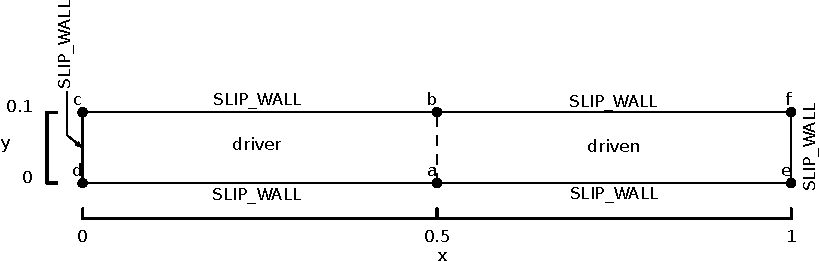
\includegraphics[width=0.9\textwidth]{../2D/classic-shock-tube/cst-edited.pdf}
\end{center}
\caption{Flow region, as modelled, for the classic shock tube.}
\label{cst-model-fig}
\end{figure}

Run the case with the following commands:\\
%
\topbar\\
\texttt{\$ cd $\sim$/cfcfd3/examples/eilmer3/2D/classic-shock-tube/}\\
\texttt{\$ ./prep\_simulation.sh}\\
\texttt{\$ ./run\_simulation.sh}\\
\texttt{\$ ./post\_simulation.sh}\\
\bottombar\\
%

The simulation is run for 100\,$\mu$s and the data is extracted for plotting against
the expected solution, as shown in Figure\,\ref{cst-profiles-fig}.
This reference solution is obtained using finite-wave and shock analysis assuming chemical equilibrium 
in the driven air.
The details of the calculation are found in Python script in Section\,\ref{finite-wave-sec}.

\begin{figure}[htbp]
\begin{tabular}{cc}
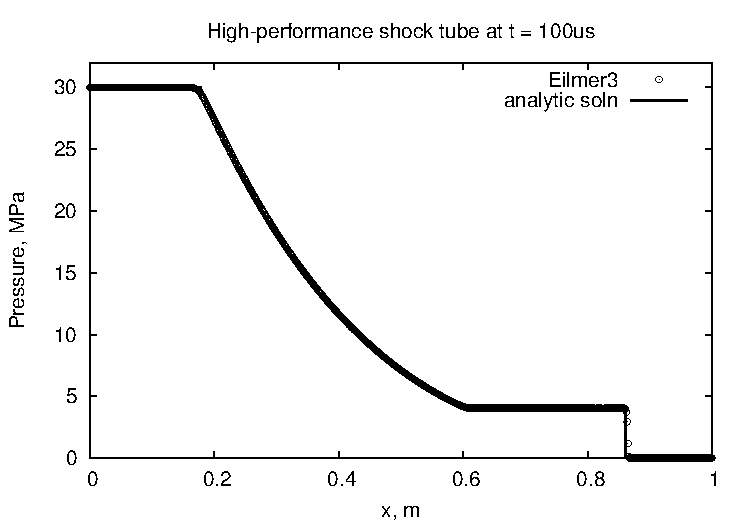
\includegraphics[width=0.5\textwidth]{../2D/classic-shock-tube/cst-p.pdf} &
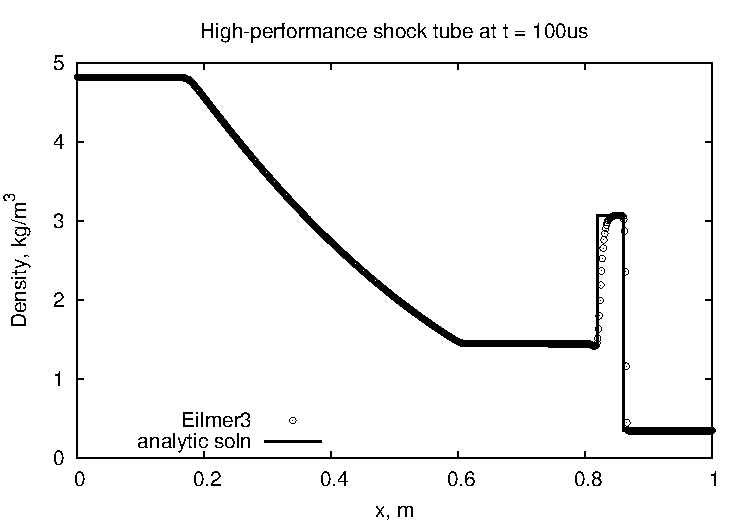
\includegraphics[width=0.5\textwidth]{../2D/classic-shock-tube/cst-rho.pdf}\\
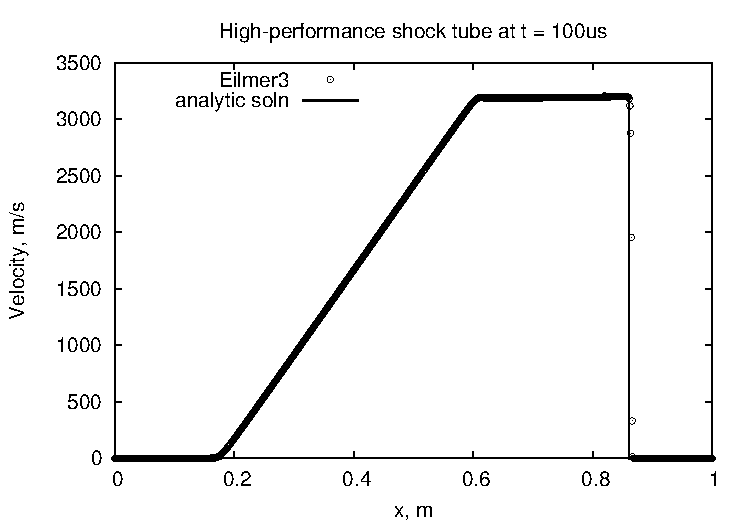
\includegraphics[width=0.5\textwidth]{../2D/classic-shock-tube/cst-u.pdf} &
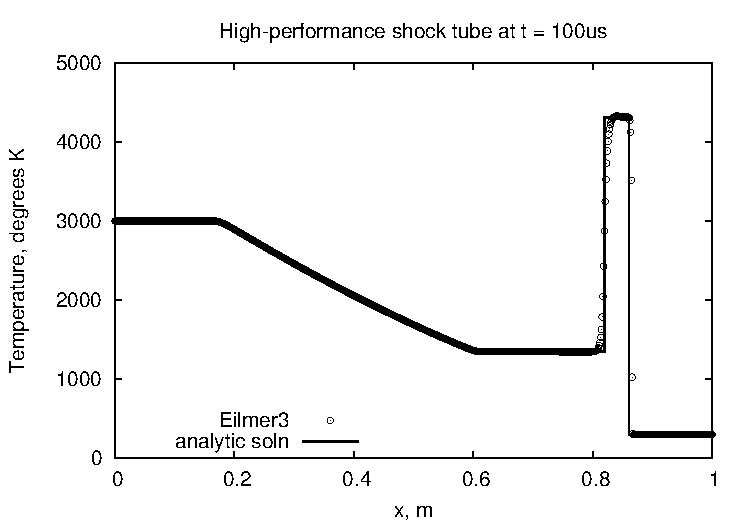
\includegraphics[width=0.5\textwidth]{../2D/classic-shock-tube/cst-T.pdf}
\end{tabular}
\caption{Flow properties along the duct for the Sod shock tube problem for nni=400.}
\label{cst-profiles-fig}
\end{figure}

Convergence of the estimated shock speed (determined by locating the pressure jump with
the \texttt{locate\_shock.py} postprocessing script) is shown in Figure\,\ref{cst-convergence-fig}.
This custom postprocessing script also computes an average of the expended driver gas speed.

\begin{figure}[htbp]
\begin{center}
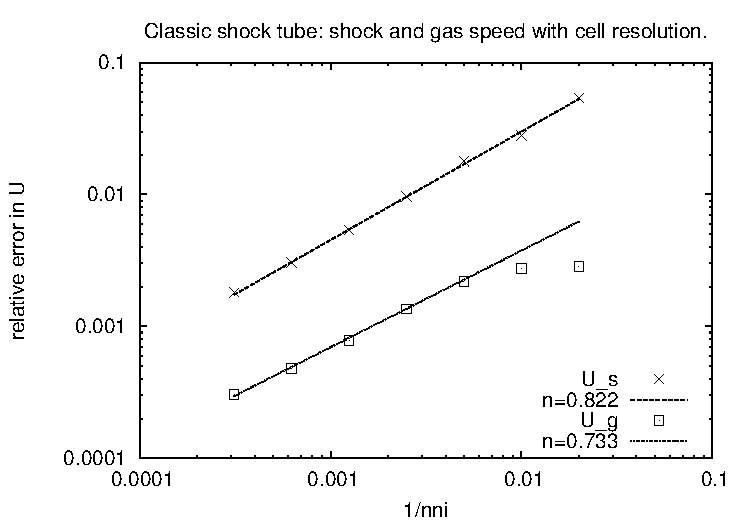
\includegraphics[width=0.6\textwidth]{../2D/classic-shock-tube/cst-errors.pdf}
\end{center}
\caption{Convergence of estimated shock speed and gas speed.}
\label{cst-convergence-fig}
\end{figure}

\newpage
\subsection{Input script (.py)}
\label{cst-py-file}
\index{gas model!look-up table!combined with composite-gas}
%
In the problem setup, below, note the combination of the look-up gas model with the composite gas model.
The helium driver gas is the only species in the composite gas and the look-up table gas models
all of the chemically-reacting species within the air test gas.
The look-up table gas ends up being prepended to the list of species for the simulation.

\noindent
\topbar
\lstinputlisting[language={}]{../2D/classic-shock-tube/cst.py}
\bottombar

\newpage
\subsection{Shell scripts}
\label{cst-sh-files}
\topbar
\lstinputlisting[language={}]{../2D/classic-shock-tube/prep_simulation.sh}
\bottombar

\noindent
\topbar
\lstinputlisting[language={}]{../2D/classic-shock-tube/run_simulation.sh}
\bottombar

\noindent
\topbar
\lstinputlisting[language={}]{../2D/classic-shock-tube/post_simulation.sh}
\bottombar

\noindent
\topbar
\lstinputlisting[language={}]{../2D/classic-shock-tube/plot_errors.sh}
\bottombar

\newpage
\subsection{Solution using finite wave and shock analysis}
\label{finite-wave-sec}
%
The NASA CEA program can be used by a library module to provide convenient estimates 
of the thermochemical state of gas mixtures at equilibrium.
The following script shows how to use that library to compute the flow for the classic
shock tube where the temperatures in the driven air test gas are large enough to 
allow significant thermochemical effects.
Beyond gas state estimation, the library provides analysis functions for simple 
flow processes such as shock and finite, isentropic waves.

\noindent
\topbar
\lstinputlisting[language={}]{../2D/classic-shock-tube/classic_shock_tube.py}
\bottombar

\newpage
\subsection{Extracting shock location and getting average gas speed}
%
\index{postprocessing!customized!shock location}
The following script is and example of how to pick up a full block of data
with the post-processing library functions and then look within that flow data
for particular features.

\noindent
\topbar
\lstinputlisting[language={}]{../2D/classic-shock-tube/locate_shock.py}
\bottombar

\subsection{Notes}
\begin{itemize}
\item The simulation with \texttt{nni = 400} takes about 13\,seconds on a recent (2011) machine 
  with an AMD Phenom 9650 quad-core processor.
\end{itemize}
